\chapter{Implementierung}
Nachdem die ersten Kontakte mit den beiden Kerntools erfolgt sind und eine geeignete Basis für das Projekt gefunden wurde, gilt es nun, dieses in die Tat umzusetzen.
Wie in \autoref{sec:einarbeitung} kann auch für das richtige Projekt eine Aufteilung der Entwicklung in Erstellung des Servers und anschließende Einbindung in das Containerimage erfolgen, was insbesondere das Testen des Servers während der Entwicklung deutlich vereinfacht und mögliche Fehlerquellen eingrenzt.

\section{Node-Server}
Angesichts dessen, dass der Node-Server im Anschluss lediglich in einen Container eingeschnürt wird, ist die Erstellung des eigentlichen Servers der deutlich größere und wichtigere Bearbeitungsschritt.
Wie bei jedem Projekt liegt auch hier der Einstiegspunkt im Errichten eines Grundgerüsts.
Im konkreten Fall bedeutet das, das node-ui5 Modul erfolgreich in Node.js zu importieren, die richtigen Konfigurationsoptionen dafür zu finden, innerhalb des Moduls den SAP Mock Server anzusteuern und diesen unkonfiguriert für externe Anfragen erreichbar zu machen.
In der Theorie klingt dies einfach.
Allerdings tritt an dieser Stelle sowohl das Problem auf, dass node-ui5 kaum dokumentiert, als auch der Mock Server nicht für solch einen Einsatz vorgesehen ist, wodurch auch die Hilfeseiten von SAP für diesen initialen Schritt nicht sonderlich hilfreich sind.

\subsection{Grundgerüst des Mock Servers}
\label{subsec:foundation}
Für das Node-Projekt wird zunächst die folgende package.json Datei (\autoref{code:basic-ms-package.json}) erstellt.
Hier wird ein Projektname mit Versionsnummer und Kurzbeschreibung angelegt, sowie in Zeile 5 der Einstiegspunkt für die Applikation definiert.
Die drei, in Zeile 6 folgende festgelegten, Projekt-Abhängigkeiten stellen hier allerdings den primär wichtigen Teil dar.
Das \enquote{body-parser}-Paket wird dafür benötigt, um den Inhalt von Anfragen an den Server sauber verarbeiten zu können.
Mit den hauseigenen Bibliotheken von Node.js ist zwar die Erstellung von Webservern bereits möglich, dieser Prozess wird jedoch vom \enquote{Express}-Framework stark vereinfacht.
Nicht zuletzt wird noch das \enquote{node-ui5}-Modul eingebunden.
Mithilfe der hier definierten Abhängigkeiten, muss nun lediglich noch \emph{npm install} ausgeführt werden und die Implementierung des Mock Servers kann starten.
\lstinputlisting[
	label=code:basic-ms-package.json,
	caption=Package.json für das Grundgerüst (gekürzt),
	captionpos=b,
	firstline=1,
	lastline=10
]{Quellcode/basic-ms/package.json}

Nachfolgend wir in \autoref{code:basic-ms-mockserver.js} der Quellcode der mockserver.js dargestellt.
Beginnend muss node-ui5 eingebunden werden (Zeile 1).
Dies geschieht hier unter Verwendung der mitgelieferten \enquote{factory}, die einige Konfigurationsschritte beim Einbinden direkt übernimmt.
Parameter, die sie dabei berücksichtigen soll, werden in den folgenden 3 Zeilen gesetzt, unter anderem die Variable \emph{myApp}, als Referenz auf das Verzeichnis, in dem die mockserver.js liegt.
Nachdem node-ui5 in Node.js eingebunden wurde, wird nun der gesamte folgende Code als Callback-Funktion der Einbindung ausgeführt.
So enthält Zeile 7 bereits SAPUI-Code, welcher weitere SAPUI-Module einbindet (hier MockServer), welche in Zeile 9 einer anschließend automatisch ausgeführten Funktion übergeben werden.

\paragraph{Konfiguration des Mock Servers}
Ab Zeile 10 wird der eigentliche Mock Server initialisiert.
Hierzu wird zunächst in der Variable \emph{ms} ein neues Mock Server Objekt erstellt, welches für den gesamten Subpfad von \enquote{/} zuständig ist.
Zeile 14 folgende teilen dem Mock Server mit, wo er die Daten findet, die er simulieren soll (myApp/mockdata), wie diese strukturiert sind (myApp/metadata.xml) und ob automatisch Platzhalter für fehlende Daten generiert werden sollen.
Zeile 19 bis 21 nehmen schließlich noch die Einstellung vor, dass der Mock Server automatisch antwortet und in diese Antwort eine künstliche Verzögerung einbaut, um die Simulation realistischer zu gestalten, bevor der Mock Server in Zeile 24 gestartet wird.

\paragraph{Externe Freigabe}
Nun läuft der Mock Server zwar und wurde mit Datensätzen versorgt, die er simulieren kann, jedoch ist er noch nicht für Anfragen außerhalb der Node.js-Umgebung erreichbar.
Zu diesem Zweck wird nun ab Zeile 26 noch ein zusätzlicher Webserver mithilfe des Express-Framework eingerichtet.
Zunächst werden hierzu die mit \ac{npm} installierten Module geladen und eine neue Express-Applikation initialisiert.
Das zusätzlich installierte Modul für den body-parser wird nun als Standardparser für Anfragen an den Express-Server konfiguriert (Zeile 30 folgende).
Anschließend wird eine Funktion festgelegt, die für jede Anfrage eines beliebigen Typs (GET, POST, PUT, ...) ausgeführt wird, die an den Express-Server geschickt werden (Zeile 35) und zwar sollen diese alle an den Mock Server weitergeleitet werden.
Der Mock Server ist so implementiert, dass er automatisch alle \ac{AJAX}-Anfragen abfängt.
Somit kann direkt basierend auf den Daten und Parametern der ursprünglichen Anfrage eine solche erstellt werden (Zeile 36-40).
Der \ac{AJAX}-Anfrage wird eine Callback-Funktion übergeben, die ausgeführt wird, wenn die Antwort des Mock Servers auf die Anfrage erfolgt ist.
In dieser werden zunächst sämtliche Header-Daten aus der \ac{AJAX}-Antwort in die Antwort des Express-Servers auf die externe Anfrage kopiert.
Letztere wird anschließend noch mit dem Status-Code der \ac{AJAX}-Response versehen und mit deren Text zurück an den externen Client geschickt (Zeile 41-51).
Übrig bleibt nur noch das Starten des Express-Servers (Zeile 56).
\lstinputlisting[
	label=code:basic-ms-mockserver.js,
	caption=Quellcode des Grundgerüsts (mockserver.js),
	captionpos=b
]{Quellcode/basic-ms/mockserver.js}

\subsection{Function Imports}
Zum aktuellen Zeitpunkt ist es bereits gelungen, einen lauffähigen \ac{OData}-Service zu errichten, welcher externe Anfragen beantwortet.
Damit dieser nun als neuer \ac{ewm-sim} dienen kann, muss er allerdings zunächst mit den richtigen Mockdaten versorgt werden.
Zu diesem Zweck muss dem Server über die \emph{metadata.xml} Datei mitgeteilt werden, wie die Datenstrukturen und Zusammenhänge zwischen diesen aussehen, die er darstellen soll.
Da der \ac{ewm-sim} eine genaue Nachbildung eines vollständigen \ac{EWM}-Systems sein soll, sind auch die Metadaten mit einem solchen übereinstimmend.
Infolge dessen kann die \emph{metadata.xml} ohne Veränderungen direkt von einem bestehenden \ac{EWM}-System übernommen werden.
Auch die darzustellenden Mockdaten haben noch dieselbe Struktur wie beim \ac{ewm-sim} in der ersten Version.
Um Mock- und Metadaten zu verändern, müssen die jeweiligen Dateien lediglich in die entsprechenden Verzeichnisse gelegt werden, welche in \autoref{subsec:foundation} konfiguriert wurden.
% \todo{Code von Meta- und Mockdaten einfügen?}

In den Metadaten werden für den vollständigen Funktionsumfang des Mock Servers jedoch überdies noch Function Imports definiert.
Diese Funktionen stellen Anfragen dar, welche erweiterte Operationen beim Server auslösen, als ausschließlich einen Datensatz zu liefern oder zu manipulieren.
Für die normalen Mockdaten benötigt der Server nicht mehr als die Daten und den entsprechenden Eintrag in den Metadaten.
Bei Function Imports funktioniert das nicht so einfach, hier ist in den Metadaten lediglich festgelegt, dass eine solche Funktion zu existieren hat, auf welche \ac{HTTP}-Methode diese reagiert, welche Parameter sie entgegennimmt und welchen Wertetyp sie zurückliefert.
Die eigentliche Funktionalität muss jedoch für jede Funktion einzeln von Hand implementiert werden.
Wie solch eine Implementierung aussieht, soll hier am Beispiel der Funktion \emph{SetRobotStatus} gezeigt werden.

\lstinputlisting[
	language=xml,
	label=code:metadata-setrobotstatus,
	caption=Metadaten der Funktion SetRobotStatus,
	captionpos=b
]{Quellcode/setrobotstatus.xml}

In \autoref{code:metadata-setrobotstatus} ist der für die Funktion relevante Ausschnitt aus der \emph{metadata.xml} zu sehen.
Diesem kann entnommen werden, dass sich die Operation der Funktion auf das \enquote{RobotSet} bezieht und die Funktion auf \ac{HTTP}-POST-Anfragen reagieren soll.
Die Funktion erwartet drei Eingabeparameter (Lgnum, Rsrc, Exccode) vom Typ String mit einer jeweils festgelegten, maximalen Länge.

Um jedoch den genauen Ablauf der Funktion im Mock Server implementieren zu können, muss die Implementierung aus dem ABAP-Backend eines richtigen \ac{EWM}-Systems analysiert und in Node.js portiert werden.
Dies ist überdies wichtig, da die importierten Funktionen bestimmte Fehlercodes zurückliefern, die für den Betrieb der Roboter ebenfalls essenziell sind.

\begin{figure}[!ht]
	\centering
	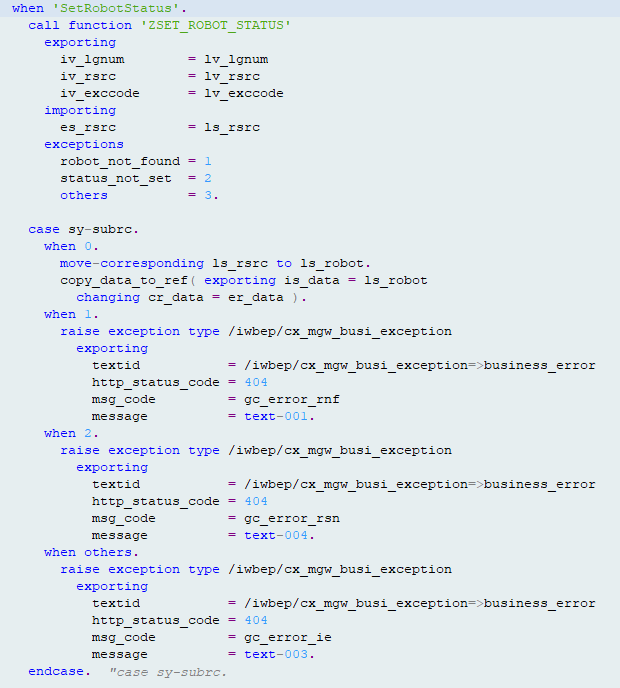
\includegraphics[width=\textwidth]{Bilder/ABAP/2020-12-04 10_20_43-Class Builder Class ZCL_ZEWM_ROBCO_DPC_EXT Display_cut.png}
	\caption{SetRobotStatus im SAP Gateway Service Builder}
	\label{fig:gwse}
\end{figure}

\autoref{fig:gwse} zeigt einen Ausschnitt aus dem \emph{SAP Gateway Service Builder}.
(Vollständige Screenshots werden aus Gründen der Lesbarkeit nicht dargestellt.)
Empfängt der \ac{OData}-Service den Aufruf von \emph{SetRobotStatus}, ruft er intern im Backend die Funktion \emph{ZSET\_ROBOT\_STATUS} mit den mitgegebenen Parametern auf.
Die Funktion kann zwei klar definierte und eine sonstige Exception zurückliefern.
Diesen Exceptions werden Exitcodes zugeordnet und anschließend wird eine Fallentscheidung anhand dieser Rückgabewerte durchgeführt.
Kommt es beispielsweise zur \emph{robot\_not\_found}-Exception, so wird vom \ac{OData}-Service eine Antwort mit dem \ac{HTTP}-Statuscode \emph{404} zurückgegeben.
Der Nachrichteninhalt wird durch die Konstante \emph{gc\_error\_rnf} festgelegt.
Um von dieser den eigentlichen Wert abzurufen, muss er im Class Builder (\autoref{fig:class-builder}) nachgeschlagen werden.
Dort steht zu jeder Konstante (Attribute) der zugehörige Wert des Fehlercodes (Initial Value).

\begin{figure}[!ht]
	\centering
	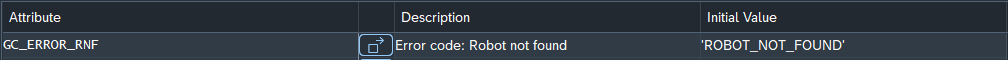
\includegraphics[width=\textwidth]{Bilder/ABAP/2020-12-04 10_22_23-Class Builder_ Display Class ZCL_ZEWM_ROBCO_DPC_EXT_cut.png}
	\caption{Fehlercodes im Class Builder}
	\label{fig:class-builder}
\end{figure}

Nun gilt es die Funktion in Node.js zu implementieren (\autoref{code:set-robot-status-method}).
Hierzu wird zunächst eine Funktion mit dem entsprechenden Namen deklariert, welche die eingehende Anfrage sowie die verwendeten URL-Parameter als Eingabewerte erhält.
Zur einfacheren Verarbeitung wird aus dem zusammenhängenden String von URL-Parametern nun ein Objekt generiert, welches Schlüssel-Wert-Paare besitzt, die entsprechend die URL-Parameter und deren Werten repräsentieren (Zeile 2-8).
Im nächsten Schritt wird überprüft, ob gemäß der übergebenen Parameter ein Roboter im Datensatz existiert, dessen Status gesetzt werden könnte.
Ist dies nicht der Fall, muss eine \emph{ROBOT\_NOT\_FOUND}-Exception zurückgegeben werden.
Die Überprüfung erfolgt über eine Anfrage an das \emph{RobotSet} desselben Servers.
Aus den URL-Parametern wird der anzufragende \ac{URI} generiert und anschließend die Anfrage ausgelöst.
Im Falle von Misserfolg der Anfrage wird die entsprechende Fehlermeldung zurückgegeben, ansonsten kann mit der Ausführung der Funktion fortgefahren werden (vergleiche Zeile 14-34).

In den Metadaten wurde für den Exccode eine maximale Länge festgelegt.
Die Einhaltung dieser muss also überprüft werden, Überschreitung der Länge ist ein Grund zum Abbruch.
Hat der übergebene Code jedoch die richtige Länge, wird erneut eine Anfrage an das servereigene \emph{RobotSet} geschickt.
Dieses Mal wird jedoch keine GET-Request geschickt, sondern mittels PUT-Request die Daten eines bestehenden Datensatzes bearbeitet.
(Durch die vorangegangene Abfrage ist sicher bekannt, dass der angefragte Roboter existiert, sonst würde diese Codestelle gar nicht ausgeführt.)
Als Payload werden schlicht und einfach die URL-Parameter in \ac{JSON}-Form verwendet.
Wird diese Anfrage erfolgreich abgeschlossen, wird die externe Anfrage mit dem Status \emph{200 OK} quittiert, andernfalls liegt ein weiterer Fehler vor.
Im \emph{SAP Gateway Service Builder} ist nur ein weiterer Fehlertyp vorgesehen.
Da der Roboter an dieser Stelle erwiesenermaßen existiert, liegt nun also der \emph{ROBOT\_STATUS\_NOT\_SET}-Fehler vor.
Dieser Fehler wird ebenfalls zurückgegeben, falls der gewünschte Status länger als die maximal erlaubte Länge sein sollte und ebenfalls in sonstigen Fehlerfällen.

\lstinputlisting[
	label=code:set-robot-status-method,
	caption=Node.js-Implementierung der Funktion SetRobotStatus,
	captionpos=b,
	firstline=1,
	lastline=64
]{Quellcode/setrobotstatus.js}

Nun existiert zwar die Funktion, ihre Existenz ist dem Mock Server jedoch noch nicht bekannt.
Um dies zu ändern, müssen zunächst die bekannten Request Handler des Mock Servers abgerufen werden.
Im Anschluss kann ihnen ein neuer Handler hinzugefügt werden, der per regulärem Ausdruck den Pfad festlegt, über den seine Funktion ausgelöst wird, auf welche Art von \ac{HTTP}-Requests er reagiert und welche Funktion er dann zurückliefern muss.
Abschließend müssen die modifizierten Request Handler noch erneut dem Mock Server bekannt gegeben werden (siehe \autoref{code:request-handler}).

\lstinputlisting[
	label=code:request-handler,
	caption=Hinzufügen des Request Handlers für die Funktion SetRobotStatus,
	captionpos=b,
	firstline=67,
	lastline=73
]{Quellcode/setrobotstatus.js}


\subsection{Authentifizierung}
Die \ac{OData}-Schnittstelle des \ac{ewm-sim} ist dafür vorgesehen, innerhalb eines Netzwerks freigegeben zu werden.
Im aktuellen Zustand wäre jeder Client in diesem Netzwerk in der Lage, nicht nur Daten von dieser Schnittstelle anzufragen, sondern diese dort auch zu manipulieren, wodurch der ordnungsgemäße Betrieb des \ac{ewm-sim} gestört werden kann.
Aus diesem Grund ist es sinnvoll, eine Authentifizierung einzubauen, die den bislang offenen Zugriff beschränkt.
Eine simple und verbreitete Methode hierfür ist \ac{HTTP}-Authentifizierung, welche, wie der Name schon sagt, direkt in \ac{HTTP} integriert ist.
Um einen Express-Server mit dieser Art der Authentifizierung zu sichern, wird lediglich ein weiteres \ac{npm}-Modul benötigt -- \emph{express-basic-auth}.
Des Weiteren muss die \emph{mockserver.js} um den in \autoref{code:basic-auth} dargestellten Code erweitert werden.
Zunächst wird hier das Modul in den Quellcode importiert (Zeile 1).
Es folgt eine Fallunterscheidung, welche überprüft, ob Zugangsdaten für den Server festgelegt worden sind.
Wie im Umfeld von Containeranwendungen üblich, werden die zu nutzenden Zugangsdaten nicht in den Quellcode integriert, sondern zum Zeitpunkt des Ausführens mittels Umgebungsvariablen festgelegt.
Dies sorgt zum einen dafür, dass für ein Ändern der Zugangsdaten nicht der Quellcode bearbeitet werden muss, zum anderen ist es somit auch unmöglich, den Server mit Standard-Anmeldedaten zu betreiben, was ein großes Sicherheitsmanko darstellen würde.
Wurden keine Zugangsdaten per Umgebungsvariable gesetzt, bricht der Server den Start ab (Zeilen 11-13).
Andernfalls wird in Zeilen 4-8 die \ac{HTTP}-Authentifizierung initialisiert.
Diese nutzt die \emph{safeCompare}-Methode der importierten Bibliothek, welche bereits gegen einige mögliche Arten von Attacken abgesichert ist, und vergleicht Nutzernamen und Passwort, die der Server bei einer Anfrage erhält, mit den in den Umgebungsvariablen festgelegten.
Stimmen beide Wertepaare überein, wird \emph{true} zurückgegeben; die Authentifizierung war erfolgreich.

\lstinputlisting[
	label=code:basic-auth,
	caption=Integration von HTTP-Authentifizierung in den Mock Server,
	captionpos=b
]{Quellcode/basic-auth.js}

\subsection{Unit-Tests}
Da der \ac{ewm-sim} bei der Entwicklung von Produktivsystemen eingesetzt werden soll, ist es von großer Bedeutung, dass er einwandfrei arbeitet.
Um dies zu gewährleisten, ist eine umfassende Überprüfung nach jeder Änderung unerlässlich.
Theoretisch könnten diese Tests händisch durchgeführt werden.
Allerdings hat eine große Software wie der im Zuge dieses Projekts erstellte Mock Server einen so ausgedehnten Funktionsumfang, dass Testungen durch einen Menschen nur stichprobenartig einzelne Funktionen überprüfen könnten.
Unit-Tests oder auch Modultests genannt bieten hingegen eine automatisierte Lösung des Testproblems.
Softwareentwickler müssen bei dieser Variante lediglich einmal solche Tests für jede zu überprüfende Funktionalität ihres Programms schreiben.
Von dort an können die Tests dann eigenständig ausgeführt werden und zeigen im Falle von Fehlern an, wo das tatsächliche Verhalten der Software vom erwarteten Ergebnis abweicht.

Modultests sind in der Softwareentwicklung sehr verbreitet, wodurch praktischerweise für eine populäre Sprache wie Node.js bereits Frameworks zur Erstellung und Durchführung solcher Tests existieren.
Eines der am weitesten verbreiteten ist \emph{Mocha} (verfügbar als \ac{npm}-Modul), mit welchem auch schon die Tests für die erste Version des \ac{ewm-sim} durchgeführt wurden.
Beides in Betracht ziehend fiel auch für die neue Version des \ac{ewm-sim} die Wahl auf Mocha, sodass auch einige bereits bestehende Tests übernommen werden konnten.
Mocha-Tests werden einfach als normale JavaScript-Datei geschrieben und in einem \enquote{test} genannten Ordner im Projektwurzelverzeichnis abgelegt.

\autoref{code:tests} zeigt einen beispielhaften Ausschnitt des Inhalts dieser Datei.
Da die Tests automatisiert laufen sollen, muss bei deren Durchführung der Mock Server ebenfalls automatisch gestartet und wieder gestoppt werden, was auch die Konfiguration der Umgebungsvariablen inkludiert, welche in den ersten drei Zeilen vorgenommen wird.
In den Zeilen 5-7 werden für die Testdurchführung benötigte Bibliotheken geladen.
Dies sind zum einen der Mock Server, eine weitere Bibliothek, die bei der Beschreibung der Testfälle benötigt wird, sowie eine aus dem ersten \ac{ewm-sim} übernommene Hilfsbibliothek, um einfach Anfragen an den Testserver schicken zu können.
Anschließend folgen die eigentlichen Tests.
Testfälle in Mocha sind entfernt dem Aufbau einer natürlichen Sprache nachempfunden.
Somit wird ein Testset mit dem Schlüsselwort \emph{\enquote{describe}} (dt. \enquote{beschreibe}) und einer menschenlesbaren Kurzbeschreibung der nachfolgenden Tests eingeleitet (Zeile 9).
Da es für automatisierte Tests üblich ist, dass gewisse Schritte vor und nach der Ausführung eines bestimmten Testfalls durchgeführt werden müssen, bringt Mocha für solches eigene Funktionen (\emph{before} und \emph{after}) mit.
Für den vorliegenden Test erfolgt in der \emph{before}-Funktion der Startvorgang des Mock Servers.
Anschließend folgen die, durch das Schlüsselwort \emph{\enquote{it}} und eine genaue Beschreibung des zu prüfenden Falls gekennzeichneten atomaren Tests.
Diese führen dann die zu testende Interaktion mit dem Server durch und vergleichen das erzielte Resultat (A) mittels der Funktion \emph{\enquote{assert.deepStrictEqual(A, B)}} mit dem erwarteten Resultat (B).
Gleichen sich die Ergebnisse exakt, war der jeweilige Test erfolgreich.

\lstinputlisting[
	label=code:tests,
	caption=Ausschnitt aus den Modultests,
	captionpos=b
]{Quellcode/tests.js}


\section{Erstellung des Dockerimages}
Nachdem der Node-Server vollständig erstellt ist und automatisiert getestet werden kann, besteht der nächste Schritt in der Einbindung in ein Dockerimage.
Der Vorgang ist nur unwesentlich komplizierter als beim in \autoref{sec:einarbeitung} beschriebenen Hello-World-Docker.
Als Besonderheit kommt hier allerdings dazu, dass das Zielimage möglichst klein sein soll.
Aufgrund von Artefakten, die beim Generieren der Node-Module entstehen, muss hier auf ein Multi-Stage-Build zurückgegriffen werden.
\Dash der Prozess der Erstellung des Dockerimages wird in mehrere Abschnitte aufgeteilt.
In \autoref{code:Dockerfile-ewm-sim} ist das entsprechende Dockerfile zu sehen.
Die erste Buildstufe wird in den Zeilen 1-5 durchlaufen.
Hierbei werden die \emph{package.json} sowie die \emph{package-lock.json} in das Arbeitsverzeichnis kopiert und dort mittels \ac{npm} die referenzierten Pakete generiert und installiert.
Anschließend wird die zweite Buildstufe (Zeilen 7-11) gestartet.
Dort werden die restlichen Projektdateien in das eigentliche Containerimage kopiert und anschließend das während der ersten Buildstufe aufgebaute Node-Modulverzeichnis aus dem ersten, temporären Image in das Zielimage kopiert.
Abschließend folgt noch die standardmäßige Freigabe des Ports \emph{8080} für den Webserver (dieser Port kann auch später noch über die Kommandozeile zur Laufzeit angepasst werden) und die Festlegung der Server-Kommandozeile, welche beim Dockerstart ausgeführt werden soll, um auch den Server hochzufahren.

\lstinputlisting[
	label=code:Dockerfile-ewm-sim,
	caption=Dockerfile für den \ac{ewm-sim},
	captionpos=b
]{Quellcode/Dockerfile}


\section{Automatisierte Tests mit Travis CI}
Wie in \autoref{sec:travis-desc} beschrieben, ist Travis CI ein häufig verwendeter Dienst, um Modultests automatisiert ausführen zu lassen, wenn der Code im Online-Repository aktualisiert wird und somit die Integrität der Software zu gewährleisten.
Für dieses Projekt wurde Travis-CI.org (eine inzwischen zugunsten der neuen Version Travis-CI.com eingestellte Variante) verwendet.
Um Tests für ein GitHub-Repository in Travis CI einzurichten, müssen zwei Dinge erledigt werden.
Zum einen muss eine Registrierung mit dem GitHub-Account, dem das Repository gehört, auf der Website von Travis CI erfolgen.
Hierbei erteilt man dem Dienst Zugriffsberechtigungen für die dem Account zugehörigen Repositories.
Anschließend wird einem von Travis CI eine Liste der auf dem Account gefundenen Repositories angezeigt, in der man mit nur einem weiteren Klick die automatische Verarbeitung für ausgewählte Repositories aktivieren kann.

Als weiterer Schritt muss Travis CI nun noch eine Konfiguration erhalten, wie die Tests für das registrierte Repository durchzuführen sind.
Diese Konfiguration erfolgt mittels der Datei \emph{\enquote{.travis.yml}}, welche im Projektwurzelverzeichnis angelegt wird.
In \autoref{code:travis.yml} ist die Konfigurationsdatei für den \ac{ewm-sim} zu sehen.
Hier wird zunächst festgelegt, in welcher Programmiersprache das Projekt geschrieben wurde und welche Version der Sprache zu verwenden ist (Zeilen 1-3).
Die \emph{install}-Sektion in Zeile 4 definiert, welche Kommandos zur Vorbereitung der Testumgebung ausgeführt werden müssen.
Im konkreten Fall müssen beispielsweise die Abhängigkeiten des Node-Servers installiert werden (Zeile 5).
Es können auch weitere Hook festgelegt werden, so zum Beispiel der in Zeile 6 aufgeführte \emph{after\_success}-Hook, der nach einer erfolgreichen Ausführung der Tests angewandt wird.
Hier wird nach den Tests noch die \enquote{Coverage} (dt. Abdeckung) bestimmt (Zeile 7).
Diese gibt an, wie groß der Anteil des Quellcodes ist, welcher von den Tests abgedeckt wird.
Eine geringe Coverage kann somit darauf hindeuten, dass nicht ausreichend Testfälle definiert wurden, um das korrekte Verhalten der Applikation zu verifizieren.
Ebenfalls in der Konfigurationsdatei festgelegt werden Benachrichtigungen (Zeile 8 fort folgende).
Für den \ac{ewm-sim} wurde dort eine E-Mail-Adresse angegeben, die im Falle von fehlgeschlagenen Tests automatisch benachrichtigt wird.

\lstinputlisting[
	label=code:travis.yml,
	caption=Konfigurationsdatei für automatisierte Tests des \ac{ewm-sim} mit Travis CI,
	captionpos=b
]{Quellcode/travis.yml}


% \section{Deployment in \ac{GKE}}
% \todo{mach ich das überhaupt noch?..}